\documentclass[10pt,a4paper]{article}

% === PAQUETES === (((
\usepackage{amsmath}
\usepackage[shortlabels]{enumitem}
\usepackage{amsfonts}
\usepackage{ragged2e}
\usepackage{subfigure}
\usepackage{amssymb}
\usepackage{slashbox}
\usepackage{multirow}
\usepackage{multicol}
\usepackage{fontspec}
\usepackage{fullpage}
\usepackage{graphicx}
\usepackage{titlesec} 
% \usepackage{setspace}
\usepackage{dsfont}
% \usepackage{bookmark}
% )))

% === TIPOGRAFÍA === (((
\setmainfont[
  BoldFont       = bodonibi,
	ItalicFont     = Century modern italic2.ttf,
	BoldItalicFont = bodonibi,
	SmallCapsFont  = lmromancaps10-regular.otf
]{Century_modern.ttf}
% )))

% === COMANDOS === (((
\newcommand{\dis}{\displaystyle}
\newcommand{\qed}{\hspace{0.5cm}\rule{0.16cm}{0.4cm}}
\newcommand{\micita}[1]{\([\)\cite{#1}\(]\)}
\newcommand{\operator}[1]{\mathop{\vphantom{\sum}\mathchoice{ \vcenter{\hbox{\huge $#1$}} }
{\vcenter{ \hbox{\Large $#1$}} }{#1}{#1}}\displaylimits}
\newcommand{\suma}{\operator{ 
\includegraphics[scale=0.09]{IMAGENES/Sigma.png}} }
\DeclareSymbolFont{italics}{\encodingdefault}{\rmdefault}{m}{it}
\DeclareSymbolFontAlphabet{\mathit}{italics}
\ExplSyntaxOn
\int_step_inline:nnnn { `A } { 1 } { `Z }
 {  \exp_args:Nf \DeclareMathSymbol{\char_generate:nn{#1}{11}}{\mathalpha}{italics}{#1} }
\int_step_inline:nnnn { `a } { 1 } { `z } {  \exp_args:Nf \DeclareMathSymbol{\char_generate:nn{#1}{11}}{\mathalpha}{italics}{#1}}
\ExplSyntaxOff
% )))

% === SECCIONES === (((
\titleformat*{\section}{\large\normalfont\bfseries}
\titleformat*{\subsection}{\large\itshape \centering}
% \setcounter{secnumdepth}{0}
\renewcommand*{\contentsname}{\large\textbf{CONTENIDOS.}}
\usepackage[nottoc,numbib]{tocbibind}
\renewcommand{\refname}{REFERENCIAS.}
\renewcommand{\tablename}{Tabla}
\renewcommand{\figurename}{Figura}
% )))

% === PORTADA === (((
% \pagestyle{empty}
\newcommand{\portada}{
\addfontfeature{LetterSpace=-5}
  \begin{titlepage}
  \centering
  \begin{figure}
    \centering
    
\includegraphics[scale=0.5]{IMAGENES/logo_uaa.png}  
  \end{figure}
  {\bfseries\Large\MakeUppercase{\textit{Universidad Autónoma de Aguascalientes.}} \par}
  \vspace{1cm}
  {\Large Centro de Ciencias Básicas. \vspace{0.5cm}\\[2mm]
  Departamento de Matemáticas y Física.\vspace{0.5cm}\\[2mm]
  Licenciatura en Matemáticas Aplicadas.\vspace{0.5cm}\\[2mm]
  Práctica 6.\par}
  \vspace{1.5cm}
  {\bfseries\Huge Experimento de Young. \par} % title
  \vspace{1.5cm}
  {\itshape\Large Óptica. \\Prof. Mariana Alfaro Gómez.\par}
  % {\itshape\Large Variable Compleja I. \\Prof. Fausto Arturo Contreras Rosales.\par}
  % {\itshape\Large Métodos Numéricos II. \\Prof. Manuel Ramírez Aranda.\par}
  % {\itshape\Large Diseño de Experimentos. \\Prof. Angélica Hernández Quintero.\par}
  % {\itshape\Large Filosofía de la Investigación Científica. \\Prof. Jesús Mariano Rodríguez Muñoz.\par}
  \vfill
  % {\Large \textit{Por Erick I. Rodríguez Juárez.}\par}
		\begin{flushleft}
		\Large
		Alumnos:\\
		\textit{Carlos Francisco Guzmán Barba.}\\
		\textit{Erick Ignacio Rodríguez Juárez.}\\
		\textit{Manuel Alejandro Siller Landin.}
		\end{flushleft}
	% {}  % {\Large \textit{Por Erick I. Rodríguez Juárez.}\par}
  \vfill
		\begin{flushright}
		{\Large Realización: 2\(/\)05\(/\)22. \par} % date
		{\Large Entrega: 16\(/\)05\(/\)22. \par} % date
		\end{flushright}
  \end{titlepage} 
	% \thispagestyle{empty}
	% \doublespacing
	% \tableofcontents
	% \singlespacing
	% \newpage
} 
% )))

\begin{document}

\portada

\section{RESUMEN.} % (((
En esta práctica  se realizaron dos experimentos cuyos objetivos fueron, correspondientemente, obtener la distancia focal de la lente y sus magnitudes dependiendo de la posición a la que se encontraba entre la fuente de luz y la pantalla. Para los experimentos, dada una lente de $10cm$ de distancia focal se obtuvo que la mejor aproximación fue de $(9.8814 \pm 0.09)cm$ y que tiene un error relativo del 1.1\textsc{\%} al generar una función que interpola a los valores experimentales obtenidos cambiando la posición de las 3 componentes (fuente de luz, lente y pantalla). Con todo esto, se pudo corroborar los hechos descritos por las ecuaciones de lentes delgadas y de magnificación, cumpliendo lo propuesto por el experimento.
% )))

\section{INTRODUCCIÓN.} % (((

\subsection{--- Marco Teórico ---} % (((
\label{sub:marco_teorico}
\begin{figure}[ht]
	\begin{minipage}{0.55\linewidth}
		\addfontfeature{LetterSpace=-5}
		Una \textbf{lente} es un objeto transparente cuya forma geométrica son dos superficies (usualmente esféricas). En la Figura \ref{fig:definicion_lente} (obtenida de \micita{alonso_finn}), se muestra una lente de dos superficies esféricas, cuyos centros son \(C_1\) y \(C_2\). \\[2mm]
		Entonces, todo rayo incidente (que no pase por la intersección de las dos superficies) tendrá dos refracciones a través del lente. \\[2mm]
		Asumiremos que los rayos \(R_1\) y \(R_2\), se transmiten en el mismo medio (como el aire), y por tanto, se tiene el mismo índice de refracción. Sea \(n\), el índice de refracción de la lente. \\[2mm]
		La recta que pasa por los puntos \(C_1\) y \(C_2\) se llama \textit{eje óptico}, y analicemos qué ocurre cuando un rayo pasa por ésta línea y por la lente, como la indica la Figura \ref{fig:incidencia}.
	\end{minipage}\hspace{5mm}
	\begin{minipage}{0.45\linewidth}
		\centering
		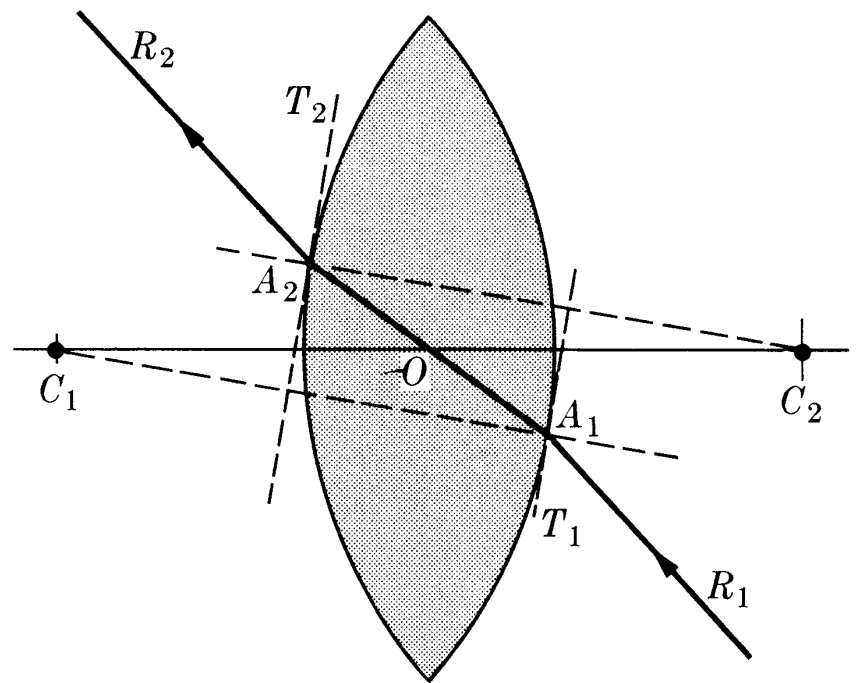
\includegraphics[width= 0.8 \linewidth]{IMAGENES/lente.png}
		\caption{Definición de lente.}
		\label{fig:definicion_lente}
	\end{minipage}
\end{figure}

\begin{figure}[ht]
	\begin{minipage}{0.5\linewidth}
		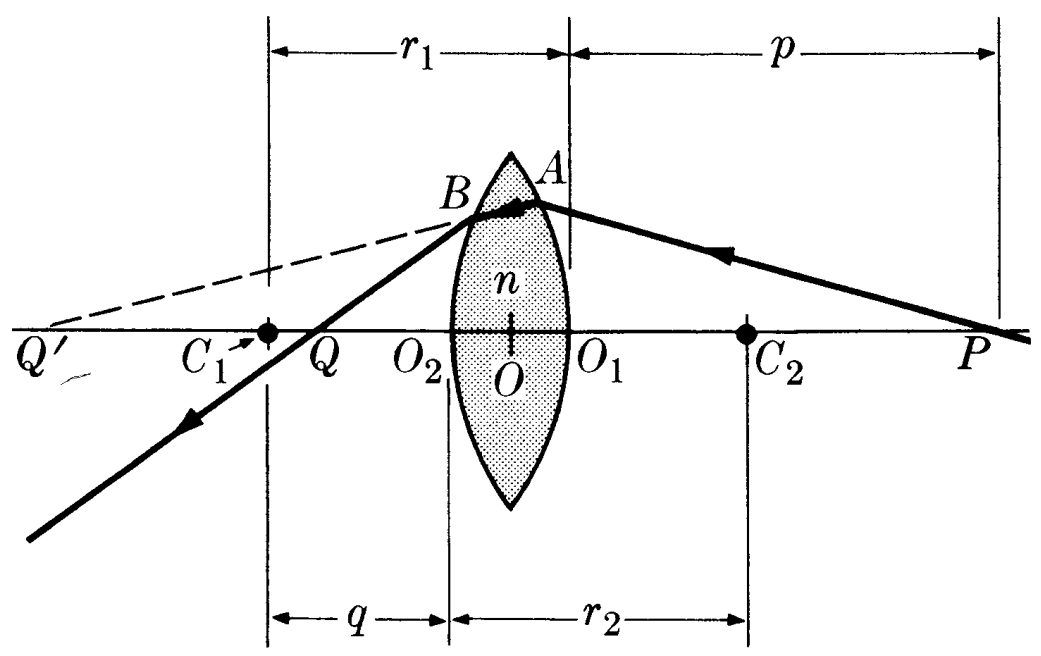
\includegraphics[width= \linewidth]{IMAGENES/incidencia.png}
		\caption{Análisis de la trayectoria de incidencia.}
		\label{fig:incidencia}
	\end{minipage}\hspace{5mm}
	\begin{minipage}{0.5\linewidth}
		\addfontfeature{LetterSpace=-5}
		Por simplicidad, se verá el comportamiento en un solo plano que pasa por \(C_1\) y \(C_2\), sin embargo, el análisis es análogo para cualquier plano en \(\mathbb{R} ^3\). \\[2mm]
		Supongamos que en la Figura \ref{fig:incidencia}, se tiene \(C_1O_1 > C_1O\). Véase \micita{alonso_finn}, para la deducción de la ecuación (\ref{eq:primera}).
		\begin{equation}
			\dfrac{1}{OP} + \dfrac{1}{OQ} = (n-1) \bigg(\dfrac{1}{r_2} - \dfrac{1}{r_1}\bigg).
			\label{eq:primera}
		\end{equation}
		La longitud de \(OP\) se llama \textit{distancia objeto}, y se representa con \(s_o\), o \(d_o\). La longitud de \(OQ\) se llama \textit{distancia imagen} y se representa con \(s_i\), o \(d_i\). \\[2mm]
	\end{minipage}
\end{figure}
Obsérvese que cuando \(P\) se mueve a la derecha en la Figura \ref{fig:incidencia}, \(OP \longrightarrow \infty\). Y así, la longitud \(OQ\) se aproxima a una distancia fija. En tal situación \(Q\) recibe el nombre de \textit{foco de la lente}, y \(OQ\) la \textit{distancia focal}, que es simétrica en ambos lados de la lente, y se denota por \(f\). Sustituyendo en (\ref{eq:primera}), se tiene la siguiente igualdad.
\[
	\dfrac{1}{OP} + \dfrac{1}{OQ} = 0+ \dfrac{1}{f} = (n-1) \bigg(\dfrac{1}{r_2} - \dfrac{1}{r_1}\bigg) \;\implies\; \dfrac{1}{f} = (n-1) \bigg(\dfrac{1}{r_2} - \dfrac{1}{r_1}\bigg).
\]
Volviendo a la expresión en (\ref{eq:primera}) con la notación descrita, obtenemos:
\begin{equation}
	\dfrac{1}{d_o} + \dfrac{1}{d_i} = \dfrac{1}{f}.
	\label{eq:ley_distancias}
\end{equation}
\newpage
Esta fórmula llamada \textit{ecuación de lentes delgadas}, permite que se puedan encontrar las distancias de las imágenes producidas por las fuentes de luz. Si \(f>0\), la lente se llama \textit{convergente}, y si \(f<0\), se llama \textit{divergente}. Las convenciones de signos se presentan en la Tabla \ref{tab:convencion_signos}, tomada de \micita{alonso_finn}.
\begin{table}[ht]
	\centering
	\caption{Convención de Signos para Superficies Esféricas Transparentes.}
	\begin{tabular}{|l|l|l|}
		\hline 
		& \hspace{7mm} \(+\) & \hspace{7mm} \(-\) \\ \hline
		Foco \(F_i\) & Convergente & Divergente \\ \hline
		Distancia Objeto \(OP\) & Real & Virtual \\ \hline
		Distancia Imagen \(OQ\) & Real & Virtual \\ \hline
		Altura Imagen \(AB\)& Vertical & Invertida \\ \hline
	\end{tabular}
	\label{tab:convencion_signos}
\end{table}\\
Así, en la Figura \ref{fig:imagen}, la obtención de la imagen que forma el objeto \(B\), queda completamente determinada en \(b\) por la intersección de dos semirayos, uno paralelo al eje óptico, y el que pasa por los puntos \(O\) y \(B\).
\begin{figure}[ht]
	\centering
	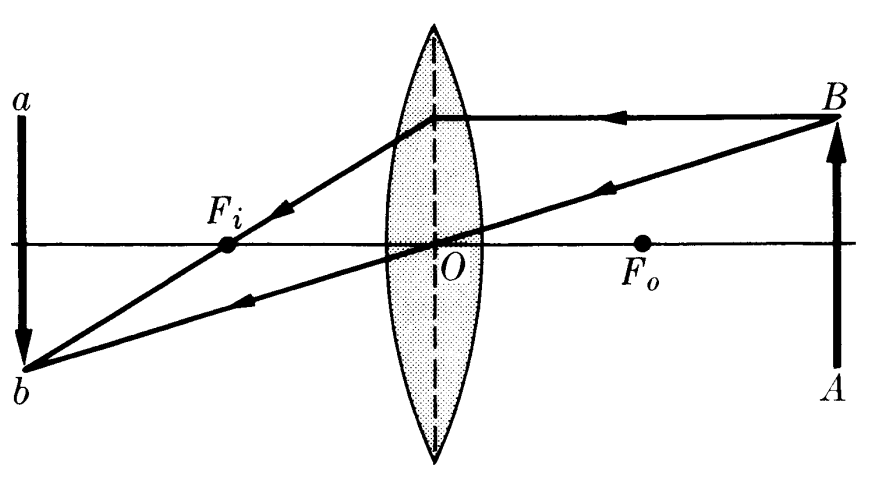
\includegraphics[width= 0.5 \linewidth]{IMAGENES/imagen.png}
	\caption{Imagen formada.}
	\label{fig:imagen}
\end{figure}\\
Se define la \textit{magnificación} de la lente, como \(M = \dfrac{ab}{AB}\).
El objetivo de los siguientes experimentos en la prática será determinar la distancia focal, y la magnificación de una lente en particular.
% )))

\subsection{--- Métodos de Análisis Experimental ---} % (((
\label{sub:analisis_exp}
Es posible obtener el foco de una lente, por medio de la intersección de dos rayos distintos, e incidentes a la superficie. Si ambos, son paralelos al eje óptico, entonces por la refracción y desviación de la lente, ambos pasarán por el foco \(F_i\) una sóla vez, así como lo indica el análisis de la sección \ref{sub:marco_teorico}. Tal procedimiento, se expone en la Figura \ref{fig:foco}.
\begin{figure}[ht]
	\centering
	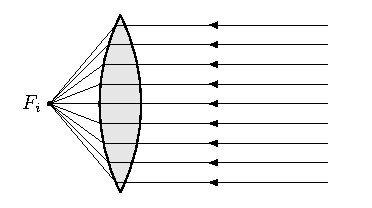
\includegraphics[width= 0.6 \linewidth]{IMAGENES/FOCO/tikz.pdf}
	\caption{Obtención experimental del foco de una lente.}
	\label{fig:foco}
\end{figure}
% )))

\subsection{--- Método de Mínimos Cuadrados ---} % (((
Sean \((x_i, y_i)\), con \(i=1, \;\ldots,\; n\), un conjunto de \(n\) puntos distintos. Se desea encontrar la recta \(f(x) =ax+b\), que minimice la suma de los cuadrados del error \(E(a,b) = \dis\suma_{i=1} ^n \big(ax_i+b -y_i\big) ^2\). Para ello, se obtiene el sistema lineal de las ecuaciones diferenciales \(\dfrac{\partial E}{\partial a} =0\), y \(\dfrac{\partial E}{\partial b} =0\). Cuyas soluciones son las siguientes.
\begin{equation}
	\begin{array}{rcl}
		a&=&\dfrac{n\left(\dis\suma_{i=1}^n x_i y_i\right)-\left(\dis\suma_{i=1}^n x_i \right)\left(\dis\suma_{i=1}^n y_i\right) }{n \left(\dis\suma_{i=1}^n x_i^2\right)-\left(\dis\suma_{i=1}^n x_i\right)^2} \\[1.6cm]
		b&=&\dfrac{\left(\dis\suma_{i=1}^n x_i^2\right)\left(\dis\suma_{i=1}^n y_i\right)-\left(\dis\suma_{i=1}^n x_i \right)\left(\dis\suma_{i=1}^n x_i y_i\right) }{n \left(\dis\suma_{i=1}^n x_i^2\right)-\left(\dis\suma_{i=1}^n x_i\right)^2}
	\end{array}
	\label{eq:intercept}
\end{equation}
Consúltese \([\)\cite{mont}\(]\), para la resolución del sistema lineal.
% )))

% )))

\section{METODOLOGÍA.} % (((

\subsection{--- Medición Directa ---} % (((
\label{sub:medicion_directa}
\begin{enumerate}[noitemsep]
	\item Se utilzó una lente convergente con una distancia focal de \(100mm\).
	\item La mínima escala del Vernier es $\dfrac{0.01 cm}{2}=0.005 cm$.
\end{enumerate}
Hablaremos sobre una forma de obtener la distancia focal de la lente mediante el uso de un objeto de tal manera que la distancia objeto entre él y la lente sea infinito o al menos muy grande (para Figura 4: Se señala la distancia a producir la imagen de uno lejano) para ello se usa el sol medir entre dos marcas características del patrón que ya que es el “objeto” más lejano que podemos enfocar pudiesen servir como referencia. de manera útil. De esta manera en un espacio que, de la luz del sol, posicionamos la lente por arriba del piso con lo que usamos el piso como nuestra pantalla para poder enfocar la lente y así medir la distancia entre la lente y el suelo obteniendo la distancia imagen del sol como se muestra en la Figura 5.
\begin{figure}[ht]
	\centering
	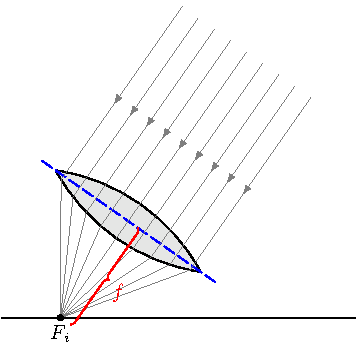
\includegraphics[height = 6cm]{IMAGENES/LUZ_SOLAR/tikz.pdf}
	\caption{Lupa inclinada arriba del suelo recibiendo la luz solar.}
	\label{fig:solar}
\end{figure}
% )))

\subsection{--- Medición de Distancias Objeto e Imagen ---} % (((
\label{sub:dist_obj_img}
La Figura \ref{fig:ima_1} y \ref{fig:ima_2} muestran la configuración para el dispositivo experimental usado. Se posiciona a \(1m\) de distancia de forma paralela la pantalla y la fuente de luz y entre ellas se coloca también de forma paralela la lente.
La mínima escala de la cinta métrica es $\dfrac{0.1 cm}{2}=0.05 cm$.
\begin{figure}[ht]
	\centering
	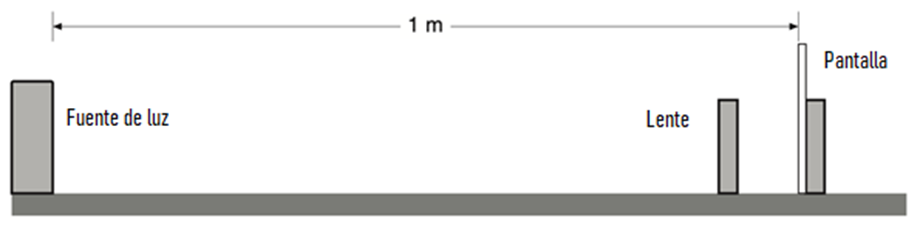
\includegraphics[width= 0.8 \linewidth]{IMAGENES/METODOLOGIA/image_1.png}
	\caption{Configuración inicial del dispositivo experimental.}
	\label{fig:ima_1}
\end{figure}\\[-5mm]
\begin{figure}[ht]
	\centering
	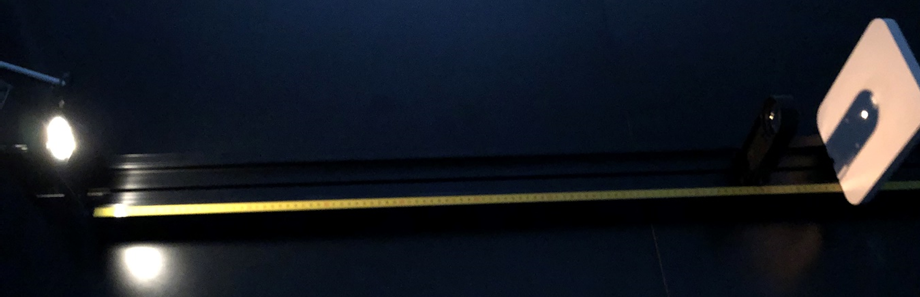
\includegraphics[width= 0.8 \linewidth]{IMAGENES/METODOLOGIA/image_2.png}
	\caption{Foto de la configuración inicial del dispositivo la cual muestra los 3 componentes ubicados de manera paralela.}
	\label{fig:ima_2}
\end{figure}\\[-3mm]
\begin{figure}[ht]
	\begin{minipage}{0.3\linewidth}
		\addfontfeature{LetterSpace=-5}
		\centering
		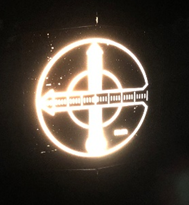
\includegraphics[height = 4.5cm]{IMAGENES/METODOLOGIA/image_3.png}
		\caption{\small La fuente de luz está intervenida por la imagen (patrón) mostrada haciendo que el objeto tenga luz propia para poder aplicar el análisis de óptica geom.}
		\label{fig:inversion}
	\end{minipage}\hspace{1cm}
	\begin{minipage}{0.5\linewidth}
		\addfontfeature{LetterSpace=-5}
		Notar que como se muestra en la Figura \ref{fig:inversion}, la fuente de luz contiene un patrón la cual al pasar por la lente podrá proyectar una imagen. \\[7mm]
		Dado que se requiere determinar la distancia focal se procede a hacer varias mediciones para después aproximar los datos mediante una función, para ello, ocupamos principalmente identificar los puntos (dos) donde la imagen proyectada desde la fuente de luz genere una imagen nítida, de ahí. \\[7mm] 
		Procedemos a obtener las mediciones de distancia objeto, distancia imagen, tamaño de la imagen en la pantalla y tamaño del objeto para 6 variaciones de la distancia entre la pantalla y la fuente de luz.
	\end{minipage}
\end{figure}
\newpage
Notar que todas las mediciones para esta sección fueron mediante el uso de un vernier dadas las pequeñas distancias y mediciones precisas requeridas. \\[2mm]
Observar que dado en la posición de la lente cercana a la fuente de luz en la que la imagen es nítida se obtendrá que sale la imagen de las dimensiones de la pantalla por lo que medir como referencia el diámetro del circulo que conforma al objeto no será factible para poder compararlo con el de la imagen, en su lugar, procedemos a medir la distancia entre dos marcas características del patrón en la imagen y en el objeto como se muestra en la Figura \ref{fig:ima_4}.
\begin{figure}[ht]
	\begin{minipage}{0.55\linewidth}
		\addfontfeature{LetterSpace=-5}
		\centering
		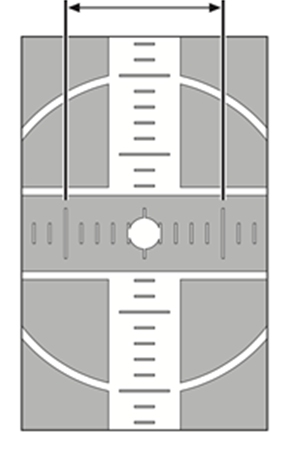
\includegraphics[height = 6cm]{IMAGENES/METODOLOGIA/image_4.png}
		\caption{Se señala la distancia a medir entre dos marcas características del patrón que pudiesen servir como referencia.}
		\label{fig:ima_4}
	\end{minipage}
	\begin{minipage}{0.45\linewidth}
		\addfontfeature{LetterSpace=-5}
		Para la posición en la que la imagen es nítida pero no sobrepasa las dimensiones de la pantalla se toma como referencia el diámetro del patrón del objeto como de la imagen. \\[1cm]
		De esta forma, para ésta sección, se obtuvieron un total de 38 mediciones; 36 fueron para las distancias objeto e imagen y para los tamaños de imagen, las 2 restantes corresponden al diámetro del circulo del patrón y a la distancia entre las marcas características de la Figura \ref{fig:ima_4}.
	\end{minipage} 
\end{figure}
% )))
\vspace{-5mm}
% )))

\section{RESULTADOS.} % (((

\subsection{--- Medición Directa ---} % (((
\label{sub:parte_1}
Se obtuvo que la distancia imagen $d_i$ del Sol (cuyos rayos se consideran paralelos al eje óptico) con la lente, era $d_i=(10.41\pm0.005)cm$. Entonces \vspace{-3mm}
$$\dfrac{1}{d_o}+\dfrac{1}{d_i}=\dfrac{1}{f} \hspace{5mm} \Longrightarrow \hspace{5mm}\dfrac{1}{\infty}+\dfrac{1}{d_i}=\dfrac{1}{f} \hspace{5mm} \Longrightarrow \hspace{5mm}  f=d_i=(10.41\pm0.005) cm $$
$$\therefore \hspace{5mm} f=(10.41\pm0.005) cm$$
% )))

\subsection{--- Medición de Distancias Objeto e Imagen ---} % (((
\label{sub:parte_2}
Los resultados de realizar las mediciones correspondientes a las distancias objeto e imagen se muestran en la Tabla \ref{tab:exp2}.
\begin{table}[ht]
	\small 
\centering
\caption{\small Distancia objeto $d_o$ y distancia imagen $d_i$ medidas en cada experimento conforme se modificaba la distancia desde la fuente de luz.}	
\begin{tabular}{|c|c|c|}
	\hline
	Distancia desde la fuente de luz (cm) & $ (d_o \pm 0.05) cm$ & $(d_i \pm 0.05)cm$ \\
	\hline
	100 & 88.9 & 11.1 \\ 	\hline
	100 & 10.2 & 89.8 \\ 	\hline
	90 & 78.9 & 11.1 \\ 	\hline
	90 & 10.4 & 79.6 \\ 	\hline
	80 & 68.6 & 11.4 \\ 	\hline
	80 & 10.5 & 69.5 \\ 	\hline
	70 & 58.5 & 11.5 \\ 	\hline
	70 & 10.8 & 59.2 \\ 	\hline
	60 & 47.85 & 12.15 \\ 	\hline
	60 & 11.3 & 48.7 \\ 	\hline
	50 & 36.65 & 13.35 \\ 	\hline
	50 & 12.2 & 37.8 \\ 	\hline
\end{tabular}
\label{tab:exp2}
\end{table}
\newpage
Luego, se calcularon los recíprocos de la distancia objeto $d_o$ y la distancia imagen $d_i$ en la Tabla \ref{tab:exp3} (el cálculo de la incertidumbre se encuentra en la sección \ref{sub:incert_part_2}).
\begin{table}[ht]
\centering
\caption{Recíprocos de las mediciones obtenidas.}		
\begin{tabular}{|c|c|c|c|c|}
	\hline & & & &\\
	Distancia $(cm)$ & $(d_o \pm 0.05) cm$ & $\dfrac{1}{(d_o \pm 0.05)} cm^{-1}$ & $(d_i \pm 0.05) cm$ & $\dfrac{1}{(d_i \pm 0.05)} cm^{-1}$ \\ & & & &\\ 	\hline
	$100$ & 88.9 & $0.0112\pm6.3265\times10^{-6}$ & 11.1 & $0.0900\pm4.0581\times10^{-4}$ \\ 	\hline
	$100$ & 10.2 & $0.0980\pm4.8058\times10^{-4}$ & 89.8 & $0.0111\pm6.2003\times10^{-6}$ \\ 	\hline
	$90$ & 78.9 & $0.0126\pm8.0318\times10^{-6}$ & 11.1 & $0.0900\pm4.0581\times10^{-4}$ \\ 	\hline
	$90$ & 10.4 & $0.0961\pm4.6227\times10^{-4}$ & 79.6 & $0.0125\pm7.8912\times10^{-6}$ \\ 	\hline
	$80$ & 68.6 & $0.0145\pm1.0624\times10^{-5}$ & 11.4 & $0.0877\pm3.8473\times10^{-4}$ \\ 	\hline
	$80$ & 10.5 & $0.0952\pm4.5351\times10^{-4}$ & 69.5 & $0.01438\pm1.0351\times10^{-5}$ \\ 	\hline
	$70$ & 58.5 & $0.0170\pm1.4610\times10^{-5}$ & 11.5 & $0.0869\pm3.7807\times10^{-4}$ \\ 	\hline
	$70$ & 10.8 & $0.0925\pm4.2866\times10^{-4}$ & 59.2 & $0.0168\pm1.4266\times10^{-5}$ \\ 	\hline
	$60$ & 47.85 & $0.0208\pm2.1837\times10^{-5}$ & 12.15 & $0.0823\pm3.3870\times10^{-4}$ \\ 	\hline
	$60$ & 11.3 & $0.0884\pm3.9157\times10^{-4}$ & 48.7 & $0.0205\pm2.1082\times10^{-5}$ \\ 	\hline
	$50$ & 36.65 & $0.0272\pm3.7223\times10^{-5}$ & 13.35 & $0.0749\pm2.8054\times10^{-4}$ \\ 	\hline
	$50$ & 12.2 & $0.0819\pm3.3593\times10^{-4}$ & 37.8 & $0.0264\pm3.4993\times10^{-5}$ \\ 	\hline
\end{tabular}
	\label{tab:exp3}
\end{table}\\
Aplicando el método de mínimos cuadrados, se obtuvo que la ecuación de la recta que mejor se ajusta a las observaciones $1/d_o$ y $1/d_i$ es
\begin{equation}
	\dfrac{1}{d_o}=(-1.0925\pm 0.0068)\left(\dfrac{1}{d_i}\right)+(0.1105\pm 0.0004)cm^{-1}
	\label{eq:regresion}
\end{equation}
Su correspondiente análisis dimensional se discute en el apéndice, sección \ref{sub:analisis_dim}.
Se grafican los datos obtenidos en la Figura \ref{fig:identidad}, junto con la recta de regresión.
\begin{figure}[ht]
\centering
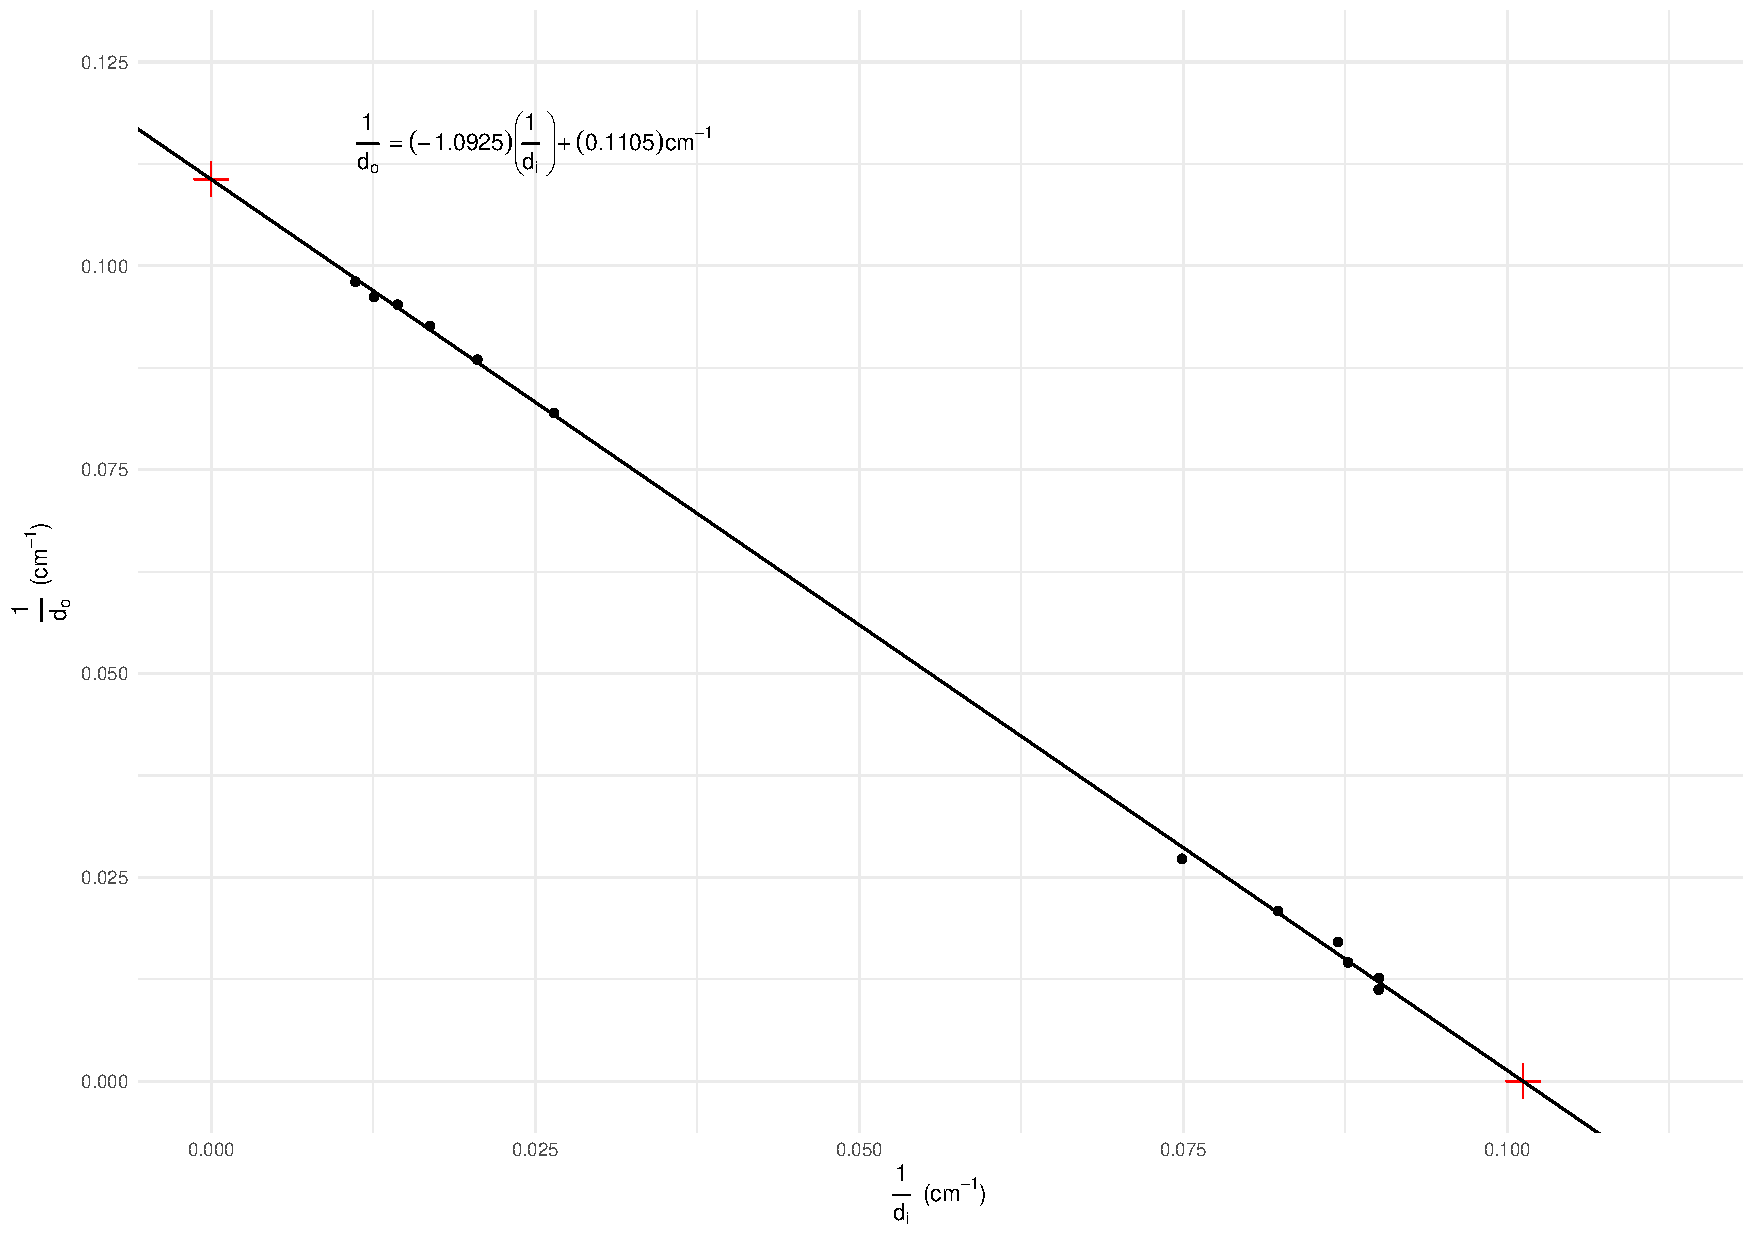
\includegraphics[width = 0.8\linewidth]{IMAGENES/graf1.pdf}
	\caption{\small \(1/d_o\) vs \(1/d_i\).}
\label{fig:identidad}
\end{figure}
\newpage
Se obtienen las intersecciones de la recta de regresión en (\ref{eq:regresion}), y el cálculo de las mismas se remite a los primeros dos puntos de la sección \ref{sub:incert_interseccion}.
\begin{multicols}{2}
\begin{itemize}
	\item Intersección con el eje de las ordenadas
	$$\dfrac{1}{d_i}=(0.1012\pm 0.0010) cm^{-1}$$
	\item Intersección con el eje de las abscisas
	$$\dfrac{1}{d_o}=(0.1105\pm 0.0004) cm^{-1} $$
\end{itemize}
\end{multicols}
Y con estos resultados se obtuvieron los datos de la Tabla \ref{tab:exp4}. Nuvamente, el cálculo de sus incetidumbres se coloca en los últimos puntos de la sección \ref{sub:incert_interseccion}.
\begin{table}[ht]
\centering
\caption{Cálculos de la distancia focal.}
\begin{tabular}{|c|c|}
\hline
Calcular a partir de: & Distancia focal \\ \hline
Intersección con eje $x$ & $(9.8814\pm0.0976)cm$\\  \hline
Intersección con eje $y$ & $(9.0497\pm 0.0818)cm$\\  \hline
Diferencia entre valores anteriores & $|9.8814-9.0497|=0.8317 $\\ \hline
Promedio de valores calculados  & $\dfrac{((9.8814+9.0497)\pm (0.0976+0.0818))cm}{2}=$\\ del eje $x$ y eje $y$ & \\
& $=(9.4655\pm 0.0897)cm$ \\ \hline
Resultado de la parte A & $(10.41\pm0.005) cm$ \\ \hline
Diferencia entre el valor calculado como & \\
el promedio de los valores del eje $x$ y eje $y$ & $|9.4655-10.41|=0.9444$ \\
y el resultado de la parte A & \\ \hline
\end{tabular}
	\label{tab:exp4}
\end{table}
% )))

\subsection{--- Estimación de la Magnificación ---} % (((
\label{sub:parte_3}
Para cada una de las distancias objeto ($d_o$) e imagen ($d_i$) se registraron los siguientes tamaño objeto ($y_o$) y tamaño imagen ($y_i$), y se colocan en la Tabla \ref{tab:parte_c}. 
\begin{table}[ht]
\centering
\caption{Tamaño objeto y tamaño imagen correspondientes a cada observación de la distancia objeto $d_o$ y distancia imagen $d_i$.}	
\begin{tabular}{|c|c|c|c|c|}
	\hline Distancia desde la&&&&\\
	 fuente de luz (cm) & $ (d_o \pm 0.05) cm$ & $(d_i \pm 0.05)cm$ & $ (y_i \pm 0.005) cm$ & $ (y_o \pm 0.005) cm$ \\ 	\hline
	100 & 88.9 & 11.1 & $-$0.54 & 4 \\ 	\hline
	100 & 10.2 & 89.8 & $-$8.18 & 1 \\ 	\hline
	90 & 78.9 & 11.1 & $-$0.83 & 4  \\ 	\hline
	90 & 10.4 & 79.6 & $-$7.02 & 1  \\ 	\hline
	80 & 68.6 & 11.4 & $-$0.7 & 4  \\ 	\hline
	80 & 10.5 & 69.5 & $-$6.02 & 1  \\ 	\hline
	70 & 58.5 & 11.5 & $-$0.83 & 4  \\ 	\hline
	70 & 10.8 & 59.2 & $-$4.925 & 1  \\ 	\hline
	60 & 47.85 & 12.15 & $-$1.03 & 4  \\ 	\hline
	60 & 11.3 & 48.7 & $-$3.9 & 1  \\ 	\hline
	50 & 36.65 & 13.35 & $-$1.7 & 4 \\ 	\hline
	50 & 12.2 & 37.8 & $-$2.845 & 1 \\ 	\hline
\end{tabular}
\label{tab:parte_c}
\end{table}
\newpage 
A partir de estos valores se calcularon los aumentos de la lente (magnificación) y su diferencia, en la Tabla \ref{tab:magnificacion}. Sus incertidumbres son obtenidas en la sección \ref{sub:incert_part_3}.
\begin{table}[ht]
\centering
\caption{Cálculo de la magnificación a partir de los datos obtenidos.}	
\begin{tabular}{|c|c|l|}
\hline &&\\
$M_1=-\dfrac{(d_i \pm 0.05) cm}{(d_o \pm 0.05)cm}$ & $M_2=\dfrac{(y_i \pm 0.05) cm}{(y_o \pm 0.05)cm}$ & $\left||M_1|-|M_2|\right|$ \\ &&\\ \hline
$-0.1248\pm0.0006$ & $-0.1350\pm0.0014$ &  $0.101$ \\ \hline
$-8.8039\pm0.0480$ & $-8.1800\pm0.0459$ &  $0.6239$ \\ \hline
$-0.1406\pm0.0007$ & $-0.2075\pm0.0015$ &  $0.668$ \\ \hline
$-7.6538\pm0.0416$ & $-7.0200\pm0.0401$ &   $0.6338$ \\ \hline
$-0.1661\pm0.0008$ & $-0.1750\pm0.0014$ &   $0.088$ \\ \hline
$-6.6190\pm0.0362$ & $-6.0200\pm0.0351$ &   $0.5990$ \\ \hline
$-0.1965\pm0.0010$ & $-0.2075\pm0.0015$ &   $0.109$ \\ \hline
$-5.4814\pm0.0300$ & $-4.9250\pm0.0296$ &   $0.5564$ \\ \hline
$-0.2539\pm0.0013$ & $-0.2575\pm0.0015$ &  $0.035$ \\ \hline
$-4.3097\pm 0.0234$ & $-3.9000\pm0.0245$ &  $0.4097$ \\ \hline
$-0.3642\pm0.0018$ & $-0.4250\pm0.0017$ &  $0.607$ \\ \hline
$-3.0983\pm0.0167$ & $-2.8450\pm0.0192$ &  $0.2533$ \\ \hline
\end{tabular}
\label{tab:magnificacion}
\end{table}	
% )))

\subsection{--- Errores de Estimación ---} % (((
\label{sub:errores}
Se exponen los márgenes de error en la Tabla \ref{tab:errores}, de las tres estimaciones de la distancia focal \(f\), obtenidas en las secciones 4.1 y 4.2.
\begin{table}[ht]
	\centering
	\caption{Cálculo de los errores con respecto al valor real \(f=10cm\).}
	\begin{tabular}{|*{4} {l|}}
		\hline 
		 & Valor (\(cm\)) & Error Absoluto (\(cm\)) & Error relativo \\ \hline
		Medición directa & \(10.41 \pm 0.005\) & 0.41 & 4.1 \textsc{\%} \\ \hline
		Intersección eje X & \(9.8814 \pm 0.09\) & 0.11 & 1.1 \textsc{\%} \\ \hline
		Intersección eje Y & \(9.0497 \pm 0.08\) & 0.95 & 9.5 \textsc{\%} \\ \hline
	\end{tabular}
	\label{tab:errores}
\end{table}
% )))

% )))

\section{DISCUSIÓN DE RESULTADOS Y CONCLUSIONES.} % (((
En el desarrollo del primer experimento, cuando se midió la distancia desde la lente a la pequeña imagen que se formaba del Sol, se obtuvo que la distancia del foco era de aproximadamente $10.41 cm$, mientras que la lente marcaba que su distancia focal era de $100mm=10 cm$, por lo que el error absoluto es tan solo del $4.1\%$ y este puede atribuirse a que tanto la persona que sostiene la lente como la que realizó la medición no son capaces de realizar el experimento sin que el pulso de sus manos no influya al sostener los instrumentos, además de que el reflejo del Sol (que en este caso se era al de medio día) también afectaba a la vista de quienes realizaban el experimento, lo que aumentó la imprecisión.  \\[2mm]
Por otro lado, en el segundo experimento donde para distintas distancias entre la lámpara y la pantalla, y conforme se hacía variar la distancia de la lente para formar imágenes nítidas, se tomaron datos de la distancia objeto $d_o$ e imagen $d_i$ así como el tamaño objeto $y_o$ e imagen $y_i$ y se pudo obtener relaciones entre distancias y tamaños. Primero se comprobó que todas las imágenes formadas por la lente en la pantalla eran reales e invertidas, lo cual era de esperarse puesto que se trataba de una lente convergente. Con las distancias objeto e imagen obtenida, se pudo obtener una estimación de la recta que pasaba por los inversos multiplicativos de estos valores, que a su vez tal estimación de la recta permitió obtener dos nuevos cálculos para la distancia focal, simplemente recabando los valores de la intersección de los ejes y calculando nuevamente los recíprocos de dichos resultados. Mediante este procedimiento se obtuvieron las diferencias absolutas entre valores considerables ($0.8317$ y $0.9444$), sin embargo, los errores absolutos comparados con la distancia focal marcada en la lente: $5.34$\textsc{\%} para el promedio de las distancias obtenidas en la intersección de las gráficas, y $4.1$\textsc{\%} (como ya se había mencionado) para el primer experimento. Aunque se esperaba que estos valores coincidieran entre sí, la principal fuente de variabilidad sigue proviniendo de la imprecisión que se tiene al realizar las mediciones así como la propagación de la incertidumbre que está asociada a los instrumentos de medición. \\[2mm]
En adición, se verifica en el apéndice \ref{sub:cuentitas}, que siempre fue posible formar con la lente dos imágenes nítidas sobre la pantalla pues $4f \leqslant k$, para $k=50,60,70,80,90,100$, lo cual se debe a que, como se discutió en el apéndice 7.6, la ecuación de segundo grado que se deriva de la fórmula de lentes delgadas siempre tiene (con las condiciones de nuestro experimento) raíces reales. Además, viendo las imágenes que se proyectaban en la pantalla, era fácil determinar que todos los “aumentos” eran negativos puesto que la imagen que generaba la lente convergente era invertida. Por último, con estos datos correspondientes a los tamaños del objeto e imagen, fue posible calcular el aumento de la lente (magnificación) sobre la imagen, y puesto que tal cálculo también está asociado con las distancias objeto e imagen, se pudo establecer el porcentaje de diferencia entre ambas relaciones, los cuales al menos no sobrepasaron el $70$\textsc{\%} de diferencia entre unidades. \\[2mm]
Así pues, determinamos la distancia focal por tres métodos distintos, cuya mejor aproximación de $(9.8814 \pm 0.09)cm$, que tiene un error relativo del 1.1\textsc{\%}, y obtuvimos su magnificación dependiendo de la posición del objeto, usando la ecuación de lentes delgadas.
% )))

% === REFERENCIAS === (((
\bibliography{Referencias}
\bibliographystyle{unsrt}
% )))

\section{APÉNDICE.} % (((

\subsection{--- Cálculo de Incertidumbres ---} % (((
\label{sub:incertidumbres}
La incertidumbre para un cociente está dada por
\begin{equation}
	\dfrac{x\pm\delta x}{y\pm\delta y}=\dfrac{x}{y}\pm\left(\dfrac{\delta x}{|y|}+|x|\dfrac{\delta y}{|y|^2}\right)
	\label{eq:cociente_incert}
\end{equation}
Consúltese \micita{incert} para la deducción de la expresión (\ref{eq:cociente_incert}).
% )))

\subsection{--- Incertidumbres de la Sección 4.2 ---} % (((
Para este caso el numerador no se trataba de una observación, sino de un número fijo, por lo que $\delta x=0$. Así pues, el cálculo de la incertidumbre para el cociente quedaría
\label{sub:incert_part_2}
\[
	\dfrac{x}{y\pm0.05}=\dfrac{x}{y}\pm|x|\dfrac{0.05}{|y|^2}
\]
	Para las observaciones de la Tabla \ref{tab:exp3}, columna 2, se tiene la distancia objeto $d_o$, y obtenemos sus recíprocos.
	\begin{align*}
		\dfrac{1}{88.9\pm 0.05}&=\dfrac{1}{88.9}\pm\dfrac{0.05}{88.9^2}=0.0112\pm6.3265\times10^{-6}\\\\
		\dfrac{1}{10.2\pm 0.05}&=\dfrac{1}{10.2}\pm\dfrac{0.05}{10.2^2}=0.0980\pm4.8058\times10^{-4}\\\\
		\dfrac{1}{78.9\pm 0.05}&=\dfrac{1}{78.9}\pm\dfrac{0.05}{78.9^2}=0.0126\pm8.0318\times10^{-6}\\\\
	\end{align*}
	\begin{align*}
		\dfrac{1}{10.4\pm 0.05}&=\dfrac{1}{10.4}\pm\dfrac{0.05}{10.4^2}=0.0961\pm4.6227\times10^{-4}\\\\
		\dfrac{1}{68.6\pm 0.05}&=\dfrac{1}{68.6}\pm\dfrac{0.05}{68.6^2}=0.0145\pm1.0624\times10^{-5}\\\\
		\dfrac{1}{10.5\pm 0.05}&=\dfrac{1}{10.5}\pm\dfrac{0.05}{10.5^2}=0.0952\pm4.5351\times10^{-4}\\\\
		\dfrac{1}{58.5\pm 0.05}&=\dfrac{1}{58.5}\pm\dfrac{0.05}{58.5^2}=0.0170\pm1.4610\times10^{-5}\\\\
		\dfrac{1}{10.8\pm 0.05}&=\dfrac{1}{10.8}\pm\dfrac{0.05}{10.8^2}=0.0925\pm4.2866\times10^{-4}\\\\
		\dfrac{1}{47.85\pm 0.05}&=\dfrac{1}{47.85}\pm\dfrac{0.05}{47.85^2}=0.0208\pm2.1837\times10^{-5}\\\\
		\dfrac{1}{11.3\pm 0.05}&=\dfrac{1}{11.3}\pm\dfrac{0.05}{11.3^2}=0.0884\pm3.9157\times10^{-4}\\\\
		\dfrac{1}{36.65\pm 0.05}&=\dfrac{1}{36.65}\pm\dfrac{0.05}{36.65^2}=0.0272\pm3.7223\times10^{-5}\\\\
		\dfrac{1}{12.2\pm 0.05}&=\dfrac{1}{12.2}\pm\dfrac{0.05}{12.2^2}=0.0819\pm3.3593\times10^{-4}
	\end{align*}
	Y para las observaciones asociadas a la distancia imagen $d_i$ (Tabla \ref{tab:exp3}, columna 4), se tiene:
	\begin{align*}
		\dfrac{1}{11.1\pm 0.05}&=\dfrac{1}{11.1}\pm\dfrac{0.05}{11.1^2}=0.0900\pm4.0581\times10^{-4}\\\\
		\dfrac{1}{89.8\pm 0.05}&=\dfrac{1}{89.8}\pm\dfrac{0.05}{89.8^2}=0.0111\pm6.2003\times10^{-6}\\\\
		\dfrac{1}{11.1\pm 0.05}&=\dfrac{1}{11.1}\pm\dfrac{0.05}{11.1^2}=0.0900\pm4.0581\times10^{-4}\\\\
		\dfrac{1}{79.6\pm 0.05}&=\dfrac{1}{79.6}\pm\dfrac{0.05}{79.6^2}=0.0125\pm7.8912\times10^{-6}\\\\
		\dfrac{1}{11.4\pm 0.05}&=\dfrac{1}{11.4}\pm\dfrac{0.05}{11.4^2}=0.0877\pm3.8473\times10^{-4}\\\\
		\dfrac{1}{69.5\pm 0.05}&=\dfrac{1}{69.5}\pm\dfrac{0.05}{69.5^2}=0.01438\pm1.0351\times10^{-5}\\\\
		\dfrac{1}{11.5\pm 0.05}&=\dfrac{1}{11.5}\pm\dfrac{0.05}{11.5^2}=0.0869\pm3.7807\times10^{-4}\\\\
	\end{align*}
	\begin{align*}
		\dfrac{1}{59.2\pm 0.05}&=\dfrac{1}{59.2}\pm\dfrac{0.05}{59.2^2}=0.0168\pm1.4266\times10^{-5}\\\\
		\dfrac{1}{12.15\pm 0.05}&=\dfrac{1}{12.15}\pm\dfrac{0.05}{12.15^2}=0.0823\pm3.3870\times10^{-4}\\\\
		\dfrac{1}{48.7\pm 0.05}&=\dfrac{1}{48.7}\pm\dfrac{0.05}{48.7^2}=0.0205\pm2.1082\times10^{-5}\\\\
		\dfrac{1}{13.35\pm 0.05}&=\dfrac{1}{13.35}\pm\dfrac{0.05}{13.35^2}=0.0749\pm2.8054\times10^{-4}\\\\
		\dfrac{1}{37.8\pm 0.05}&=\dfrac{1}{37.8}\pm\dfrac{0.05}{37.8^2}=0.0264\pm3.4993\times10^{-5}\\\\
	\end{align*}
% )))

	\subsection{--- Análisis Dimensional de la Sección 4.2 ---} % (((
	\label{sub:analisis_dim}
	Las unidades correspondientes a todos los cálculos anteriores serían $$\left[\dfrac{1}{d_o}\right]=\left[\dfrac{1}{d_i}\right]=\dfrac{1}{cm}=cm^{-1}$$
	Para la pendiente
	\begin{align*}
		[a]&=\dfrac{n\displaystyle\suma_{i=1}^{n}\left[\dfrac{1}{d_i}\right]\left[\dfrac{1}{d_o}\right]-\displaystyle\suma_{i=1}^{n}\left[\dfrac{1}{d_i}\right]\displaystyle\suma_{i=1}^{n}\left[\dfrac{1}{d_o}\right]}{n\displaystyle\suma_{i=1}^{n}\left[\dfrac{1}{d_i}\right]^2-\left(\displaystyle\suma_{i=1}^{n}\left[\dfrac{1}{d_i}\right]\right)^2}=\\\\
		&=\dfrac{cm^{-1}\cdot cm^{-1}-cm^{-1}\cdot cm^{-1}}{cm^{-2}-cm^{-2}}=\dfrac{cm^{-2}}{cm^{-2}}=1
	\end{align*}
	lo que muestra que la pendiente es un número adimensional. 
	
	Para la ordenada al origen
	\begin{align*}
		[b]&=\dfrac{n\displaystyle\suma_{i=1}^{n}\left[\dfrac{1}{d_i}\right]^2\displaystyle\suma_{i=1}^{n}\left[\dfrac{1}{d_o}\right]-\displaystyle\suma_{i=1}^{n}\left[\dfrac{1}{d_i}\right]\displaystyle\suma_{i=1}^{n}\left[\dfrac{1}{d_i}\right]\left[\dfrac{1}{d_o}\right]}{n\displaystyle\suma_{i=1}^{n}\left[\dfrac{1}{d_i}\right]^2-\left(\displaystyle\suma_{i=1}^{n}\left[\dfrac{1}{d_i}\right]\right)^2}=\\\\
		&=\dfrac{cm^{-2}\cdot cm^{-1}-cm^{-1}\cdot cm^{-1}\cdot cm^{-1}}{cm^{-2}-cm^{-2}}=\dfrac{cm^{-3}}{cm^{-2}}=cm^{-1}
	\end{align*}
	$$\therefore \hspace{5mm} [b]= cm^{-1}$$
	% )))

\subsection{--- Intersecciones e Incertidumbres de la Recta de Regresión ---} % (((
\label{sub:incert_interseccion}
	\begin{itemize}
		\item Para la intersección con el eje de las ordenadas, como se tiene que la ecuación de la recta es $(a\pm \Delta a)x+(b\pm \Delta b)$, entonces
		$$(a\pm \Delta a)x+(b\pm \Delta b)=0\Longleftrightarrow x=\dfrac{(-b\pm \Delta b)}{(a\pm \Delta a)} $$ 
		
			Con los valores estimados y la fórmula de la propagación de la incertidumbre (\ref{eq:cociente_incert}), obtenemos
		\begin{align*}
			\dfrac{1}{d_i}&=\dfrac{(-0.1105\pm 0.0004) cm^{-1}}{(-1.0925\pm 0.0068)}=
			\dfrac{0.1105 cm^{-1}}{1.0925}\pm\left(\dfrac{0.0004 cm^{-1}}{1.0925}+(0.1105 cm^{-1})\cdot \dfrac{0.0068}{1.0925^2}\right)=\\\\
			&=(0.1012\pm 0.0010) cm^{-1}
		\end{align*}
	
		\item Para la intersección con el eje de las abscisas, tal valor es el correspondiente a $b\pm \Delta b$ de la ecuación de la recta, por lo que se tiene que
		$$\dfrac{1}{d_o}=(0.1105\pm 0.0004) cm^{-1} $$
	\end{itemize}
	
	Luego, para el cálculo de las distancias focales, se tiene
	\begin{itemize}
		\item  Con el valor de la intersección con el eje de las ordenadas
		$$\dfrac{1}{(0.1012\pm 0.0010) cm^{-1}}=\left(\dfrac{1}{0.1012}\pm\dfrac{0.0010}{0.1012^2}\right)cm=(9.8814\pm0.0976)cm$$
		
		\item  Con el valor de la intersección con el eje de las abscisas
		$$\dfrac{1}{(0.1105\pm 0.0004) cm^{-1}}=\left(\dfrac{1}{0.1105}\pm\dfrac{0.0010}{0.1105^2}\right)cm=(9.0497\pm 0.0818)cm$$
	\end{itemize}
% )))

\subsection{--- Incertidumbres de la Magnificación ---} % (((
\label{sub:incert_part_3}
	De la fórmula de la propagación de incertidumbre (\ref{eq:cociente_incert}), para los datos de la distancia objeto ($d_o$) e imagen ($d_i$) (Tabla 5, columnas 2 y 3), se obtuvo lo siguiente
	\begin{align*}
		-\dfrac{(11.1\pm 0.05)cm}{(88.9\pm 0.05)cm}&=-\dfrac{11.1}{88.9}\pm\left(\dfrac{0.05}{88.9}+11.1\cdot\dfrac{0.05}{88.9^2}\right)=-0.1248\pm0.0006\\\\
		-\dfrac{(89.8\pm 0.05)cm}{(10.2\pm 0.05)cm}&=-\dfrac{89.8}{10.2}\pm\left(\dfrac{0.05}{10.2}+89.8\cdot\dfrac{0.05}{10.2^2}\right)=-8.8039\pm0.0480\\\\
		-\dfrac{(11.1\pm 0.05)cm}{(78.9\pm 0.05)cm}&=-\dfrac{11.1}{78.9}\pm\left(\dfrac{0.05}{78.9}+11.1\cdot\dfrac{0.05}{78.9^2}\right)=-0.1406\pm0.0007\\\\
		-\dfrac{(79.6\pm 0.05)cm}{(10.4\pm 0.05)cm}&=-\dfrac{79.6}{10.4}\pm\left(\dfrac{0.05}{10.4}+79.6\cdot\dfrac{0.05}{10.4^2}\right)=-7.6538\pm0.0416\\\\
		-\dfrac{(11.4\pm 0.05)cm}{(68.6\pm 0.05)cm}&=-\dfrac{11.4}{68.6}\pm\left(\dfrac{0.05}{68.6}+11.4\cdot\dfrac{0.05}{68.6^2}\right)=-0.1661\pm0.0008\\\\
		-\dfrac{(69.5\pm 0.05)cm}{(10.5\pm 0.05)cm}&=-\dfrac{69.5}{10.5}\pm\left(\dfrac{0.05}{10.5}+69.5\cdot\dfrac{0.05}{10.5^2}\right)=-6.6190\pm0.0362
	\end{align*}
	\begin{align*}
		-\dfrac{(11.5\pm 0.05)cm}{(58.5\pm 0.05)cm}&=-\dfrac{11.5}{58.5}\pm\left(\dfrac{0.05}{58.5}+11.5\cdot\dfrac{0.05}{58.5^2}\right)=-0.1965\pm0.0010\\\\
		-\dfrac{(59.2\pm 0.05)cm}{(10.8\pm 0.05)cm}&=-\dfrac{59.2}{10.8}\pm\left(\dfrac{0.05}{10.8}+59.2\cdot\dfrac{0.05}{10.8^2}\right)=-5.4814\pm0.0300\\\\
		-\dfrac{(12.15\pm 0.05)cm}{(47.85\pm 0.05)cm}&=-\dfrac{12.15}{47.85}\pm\left(\dfrac{0.05}{47.85}+12.15\cdot\dfrac{0.05}{47.85^2}\right)=-0.2539\pm0.0013\\\\
		-\dfrac{(48.7\pm 0.05)cm}{(11.3\pm 0.05)cm}&=-\dfrac{48.7}{11.3}\pm\left(\dfrac{0.05}{11.3}+48.7\cdot\dfrac{0.05}{11.3^2}\right)=-4.3097\pm 0.0234\\\\
		-\dfrac{(13.35\pm 0.05)cm}{(36.65\pm 0.05)cm}&=-\dfrac{13.35}{36.65}\pm\left(\dfrac{0.05}{36.65}+13.35\cdot\dfrac{0.05}{36.65^2}\right)=-0.3642\pm0.0018\\\\
		-\dfrac{(37.8\pm 0.05)cm}{(12.2\pm 0.05)cm}&=-\dfrac{37.8}{12.2}\pm\left(\dfrac{0.05}{12.2}+37.8\cdot\dfrac{0.05}{12.2^2}\right)=-3.0983\pm0.0167
	\end{align*}
	y con los datos del tamaño objeto e imagen (Tabla 5, columnas 4 y 5) se obtuvo  
	\begin{align*}
		\dfrac{(-0.54\pm0.005)cm}{(4\pm0.005)cm}&=\dfrac{-0.54}{4}\pm\left(\dfrac{0.005}{4}+0.54\cdot\dfrac{0.005}{4^2}\right)=-0.1350\pm0.0014\\\\
		\dfrac{(-8.18\pm0.005)cm}{(1\pm0.005)cm}&=\dfrac{-8.18}{1}\pm\left(\dfrac{0.005}{1}+8.18\cdot\dfrac{0.005}{1^2}\right)=-8.1800\pm0.0459\\\\
		\dfrac{(-0.83\pm0.005)cm}{(4\pm0.005)cm}&=\dfrac{-0.83}{4}\pm\left(\dfrac{0.005}{4}+0.83\cdot\dfrac{0.005}{4^2}\right)=-0.2075\pm0.0015\\\\
		\dfrac{(-7.02\pm0.005)cm}{(1\pm0.005)cm}&=\dfrac{-7.02}{1}\pm\left(\dfrac{0.005}{1}+7.02\cdot\dfrac{0.005}{1^2}\right)=-7.0200\pm0.0401\\\\
		\dfrac{(-0.7\pm0.005)cm}{(4\pm0.005)cm}&=\dfrac{-0.7}{4}\pm\left(\dfrac{0.005}{4}+0.7\cdot\dfrac{0.005}{4^2}\right)=-0.1750\pm0.0014\\\\
		\dfrac{(-6.02\pm0.005)cm}{(1\pm0.005)cm}&=\dfrac{-6.02}{1}\pm\left(\dfrac{0.005}{1}+6.02\cdot\dfrac{0.005}{1^2}\right)=-6.0200\pm0.0351\\\\
		\dfrac{(-0.83\pm0.005)cm}{(4\pm0.005)cm}&=\dfrac{-0.83}{4}\pm\left(\dfrac{0.005}{4}+0.83\cdot\dfrac{0.005}{4^2}\right)=-0.2075\pm0.0015\\\\
		\dfrac{(-4.925\pm0.005)cm}{(1\pm0.005)cm}&=\dfrac{-4.925}{1}\pm\left(\dfrac{0.005}{1}+4.925\cdot\dfrac{0.005}{1^2}\right)=-4.9250\pm0.0296
	\end{align*}
	\begin{align*}
		\dfrac{(-1.03\pm0.005)cm}{(4\pm0.005)cm}&=\dfrac{-1.03}{4}\pm\left(\dfrac{0.005}{4}+1.03\cdot\dfrac{0.005}{4^2}\right)=-0.2575\pm0.0015\\\\
		\dfrac{(-3.9\pm0.005)cm}{(1\pm0.005)cm}&=\dfrac{-3.9}{1}\pm\left(\dfrac{0.005}{1}+3.9\cdot\dfrac{0.005}{1^2}\right)=-3.9000\pm0.0245\\\\
		\dfrac{(-1.7\pm0.005)cm}{(4\pm0.005)cm}&=\dfrac{-1.7}{4}\pm\left(\dfrac{0.005}{4}+1.7\cdot\dfrac{0.005}{4^2}\right)=-0.4250\pm0.0017\\\\
		\dfrac{(-2.845\pm0.005)cm}{(1\pm0.005)cm}&=\dfrac{-2.845}{1}\pm\left(\dfrac{0.005}{1}+2.845\cdot\dfrac{0.005}{1^2}\right)=-2.8450\pm0.0192
	\end{align*}
% )))

	\subsection{--- Posiciones Nítidas en el Experimento ---} % (((
	\label{sub:cuentitas}
	Notamos que, por las propiedades de la lente, en la ecuación (\ref{eq:ley_distancias}),
	\[
		\dfrac{1}{d_i} + \dfrac{1}{d_o} = \dfrac{1}{f}.
	\]
	Por las propiedades del experimento, tendremos la pantalla de forma fija, a una distancia \(k\), de la fuente de luz, \textit{i.e.}
	\begin{equation}
		d_i+d_o = k
		\label{eq:fija}
	\end{equation}
	Por tanto
	\[
		\begin{array}{rcl}
			&&\hspace{-2.65cm} \left\{ \begin{array}{rcl}
				d_i & = & k-d_o \\[2mm]
			\dfrac{1}{d_i} + \dfrac{1}{d_o} &= &  \dfrac{1}{f}.
		\end{array}\right. \\[1cm]
			\therefore \hspace{5mm} \dfrac{d_o+(k-d_o)}{(k-d_o) d_o} & = & \dfrac{1}{f} \\[7mm]
			\therefore \hspace{5mm} \dfrac{(k-d_0) d_0}{d_0+(k-d_0)} & = & f \\[7mm]
			\therefore \hspace{5mm} \dfrac{(k-d_0) d_o}{k} & = & f \\[7mm]
			\therefore \hspace{5mm} kd_0-d_o^2 & = & kf.
		\end{array}
	\]
	Consecuentemente, se tendrá:
	\[
		\fbox{\(d_o^2-kd_o+kf =0\)}
	\]
	Luego,
	\[
		d_o = \dfrac{-(-k) \pm \sqrt{k^2-4(1)(kf)}}{2(1)} = \dfrac{k \pm \sqrt{k^2-4kf}}{2}.
	\]
	Esto indica que existen exactamente dos posiciones en las que se formará la imagen a una distancia objeto fija, a saber,
	\[
		\begin{array}{rcl}
			d_o & = & \dfrac{k + \sqrt{k^2-4kf}}{2} \\[7mm]
			d_o & = & \dfrac{k - \sqrt{k^2-4kf}}{2}
		\end{array}
	\]
	siempre y cuando \(k^2-4kf \geqslant 0\), es decir, \(k \geqslant 4f\).
	% )))

% )))

\end{document}
